\documentclass[tikz,border=10pt]{standalone}
\usepackage{tikz}
\usetikzlibrary{patterns, arrows.meta, positioning, calc}

\begin{document}
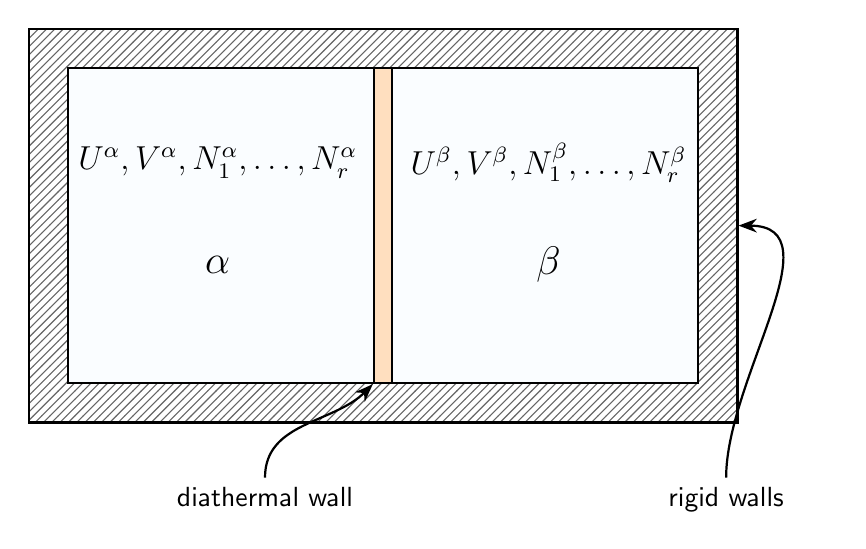
\begin{tikzpicture}
    % --- Style Definitions ---
    \tikzset{
        % Rigid outer wall (insulation)
        wall style/.style={
            draw=black, 
            thick, 
            pattern=north east lines, 
            pattern color=black!60
        },
        % The gas/subsystems background
        system fill/.style={
            fill=cyan!2
        },
        % The diathermal wall (heat conducting)
        diathermal style/.style={
            fill=orange!25,
            draw=black,
            thick
        },
        % Text styling
        label text/.style={
            font=\sffamily, 
            color=black
        },
        math text/.style={
            font=\large
        },
        % Arrow styling
        annotation arrow/.style={
            ->, 
            >=Stealth, 
            thick, 
            black
        }
    }

    % --- 1. Draw the Walls (Outer Box) ---
    % Width increased slightly to accommodate the two chambers
    \node[
        wall style, 
        minimum width=9cm, 
        minimum height=5cm
    ] (outer) at (0,0) {};

    % --- 2. Draw the Inner Chamber Background ---
    % We draw a white/cyan box over the pattern to create the empty space
    \node[
        system fill, 
        draw=black, 
        thick, 
        minimum width=8cm, 
        minimum height=4cm
    ] (inner) at (0,0) {};

    % --- 3. Draw the Diathermal Wall (Divider) ---
    % A thin vertical rectangle in the center
    \node[
        diathermal style, 
        minimum width=0.2cm, 
        minimum height=4cm,
        anchor=center
    ] (divider) at (0,0) {};

    % --- 4. System Variables (Alpha Side - Left) ---
    % Using relative coordinates from the center of the left half
    \node[math text] at (-2.1, 0.8) {$U^\alpha, V^\alpha, N_1^\alpha, \dots, N_r^\alpha$};
    \node[font=\Large] at (-2.1, -0.5) {$\alpha$};

    % --- 5. System Variables (Beta Side - Right) ---
    \node[math text] at (2.1, 0.8) {$U^\beta, V^\beta, N_1^\beta, \dots, N_r^\beta$};
    \node[font=\Large] at (2.1, -0.5) {$\beta$};

    % --- 6. Annotations ---

    % Annotation: Diathermal Wall
    \node[label text, anchor=north] (lbl_dia) at (-1.5, -3.2) {diathermal wall};
    % Arrow curving up to the center divider
    \draw[annotation arrow] (lbl_dia.north) to[out=90, in=225] (divider.south west);

    % Annotation: Rigid Walls
    \node[label text, anchor=north west] (lbl_wall) at (3.5, -3.2) {rigid walls};
    % Arrow pointing to the outer patterned boundary
    \draw[annotation arrow] (lbl_wall.north) to[out=90, in=0] (outer.east);

\end{tikzpicture}
\end{document}